
\begin{figure}[h]
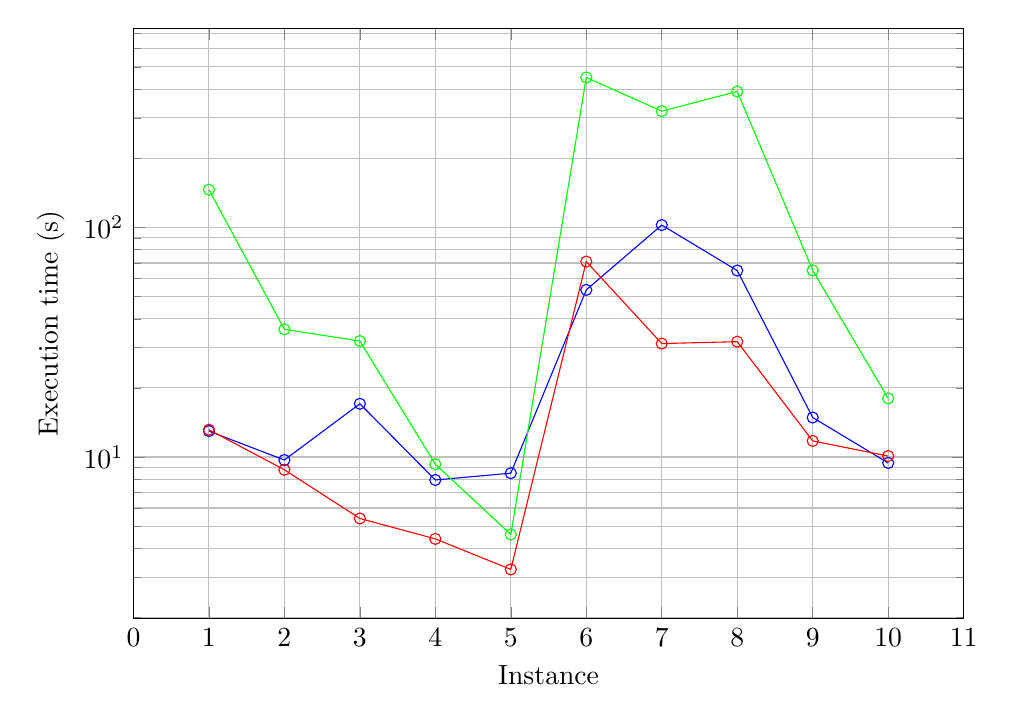
\begin{tikzpicture}
	\begin{axis}[width=\textwidth,height=60ex,
		xlabel=Instance,
		ylabel=Execution time (s), xmin=0, ymin=0, grid=both,
		ymode=log]
	
	
\addplot[mark=o,color=blue] coordinates {
(1, 12.96708331)
(2, 9.704563172)
(3, 17.056811547)
(4, 7.944795782)
(5, 8.505190252)
(6, 53.456992427)
(7, 102.392618933)
(8, 64.881486922)
(9, 14.86064378)
(10, 9.421963416)
};

\addplot[mark=o,color=red] coordinates {
(1, 13.152454848)
(2, 8.8)
(3, 5.4)
(4, 4.4)
(5, 3.24)
(6, 70.99)
(7, 31.2)
(8, 31.8)
(9, 11.75)
(10, 10.1)
};


\addplot[mark=o,color=green] coordinates {
(1, 146)
(2, 36)
(3, 32)
(4, 9.3)
(5, 4.6)
(6, 450.1)
(7, 321)
(8, 391)
(9, 65)
(10, 18)
};

\end{axis}

\end{tikzpicture}%
\caption{Execution time for Gurobi on all instances with P1 (in red) and P3 (in blue) and for Cbc with P1, without any optimization (in green). Cbc with P3 would take too much time and we would often not see the end of the computation, it is therefore not relevant to display it here along the others.}
\end{figure}
